%First stage



\begin{figure}[htbp]
    \centering
    
    \begin{subfigure}{\textwidth}
        \centering
        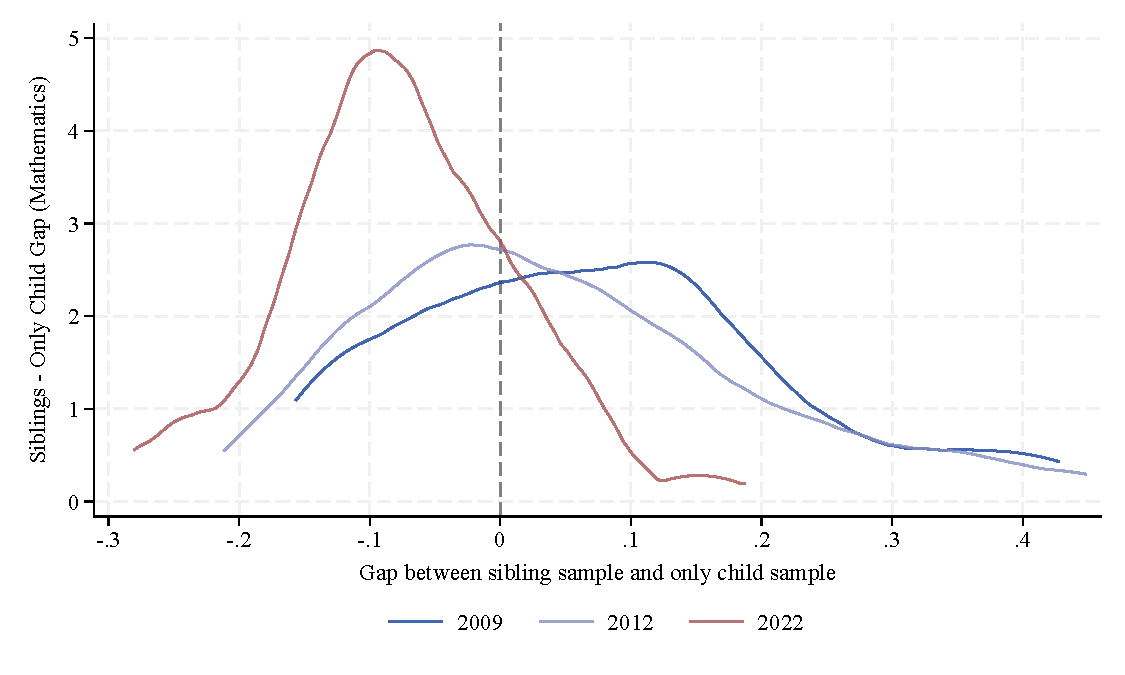
\includegraphics[width=\textwidth]{./FIGURES/Descriptive/PISA_gap_PV1MATH_histogram_2009_2022.pdf}
        \caption{Learning gaps in Mathematics by year}
        \label{fig:1a}
    \end{subfigure}
    
    \vspace{1em} % Add some vertical space between subfigures
    
    \begin{subfigure}{\textwidth}
        \centering
        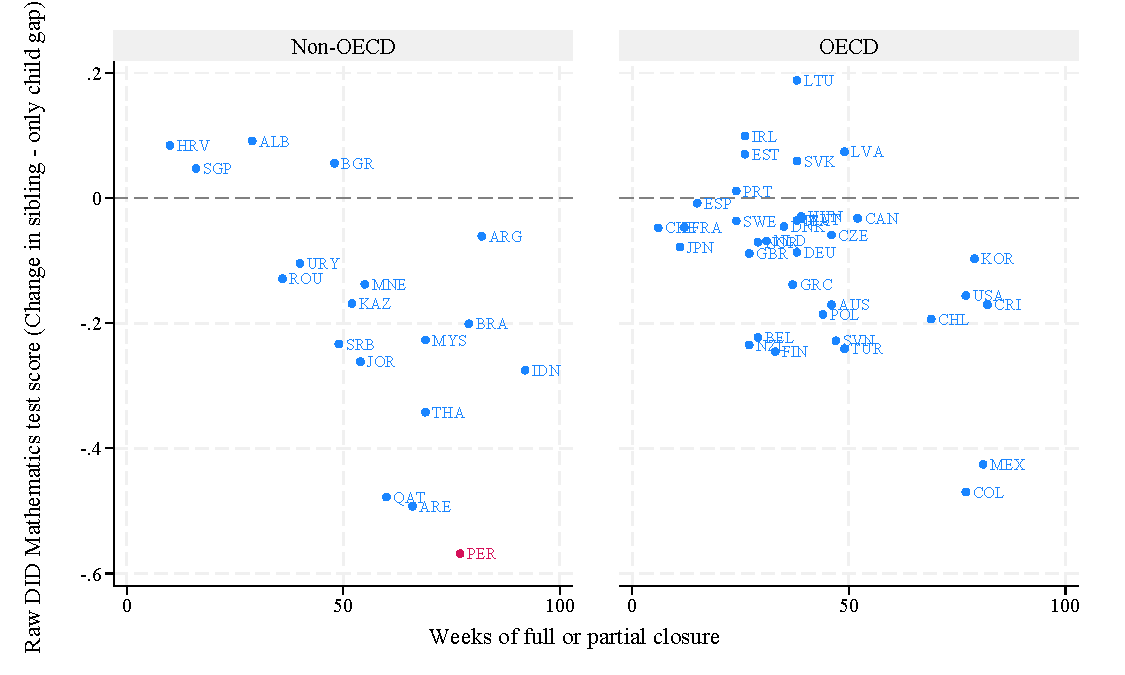
\includegraphics[width=\textwidth]{./FIGURES/Descriptive/PISA_raw_DID_PV1MATH_not_fully_open.pdf}
        \caption{Change in learning gaps by duration of school closure for OECD and Non-OECD countries.}
        \label{fig:1b}
    \end{subfigure}
    
    \caption{Learning gaps around the world}
    \label{fig:pisa}
\end{figure}


\begin{figure}[htbp]
    \centering
    
    \begin{subfigure}{\textwidth}
        \centering
        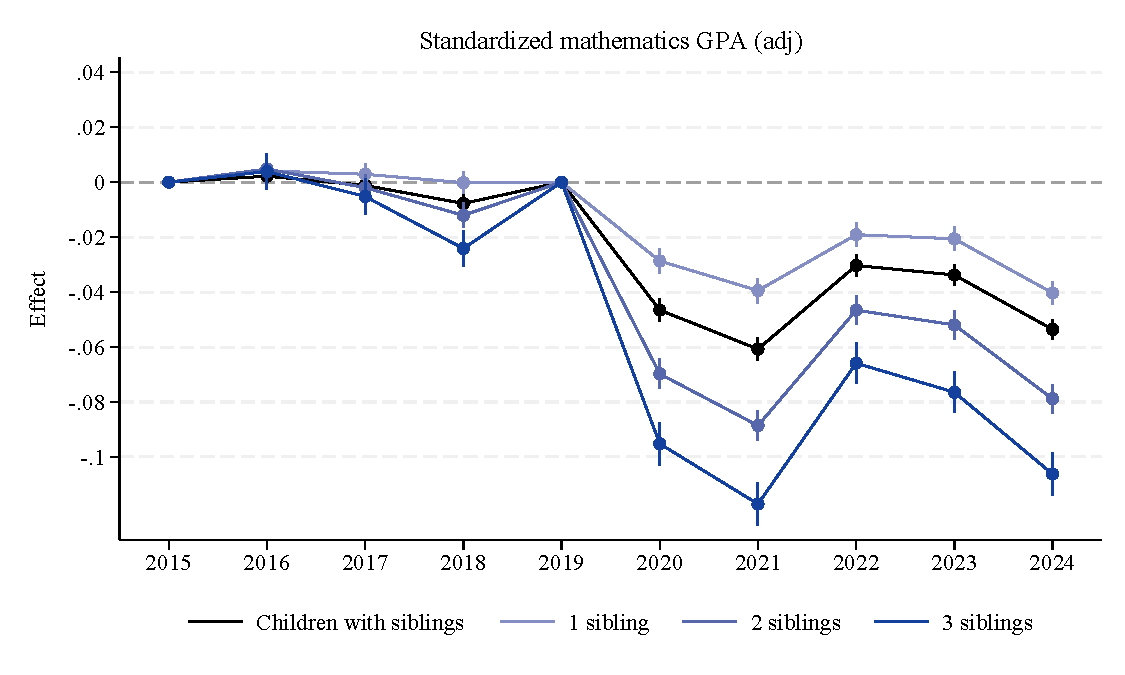
\includegraphics[width=\textwidth]{./FIGURES/Event Study/covid_std_gpa_m_adj_all_all_all_elm_all.pdf}
        \caption{Event Study}
        \label{fig:fig2a}
    \end{subfigure}
    
    \vspace{1em} % Add some vertical space between subfigures
    
    \begin{subfigure}{\textwidth}
        \centering
        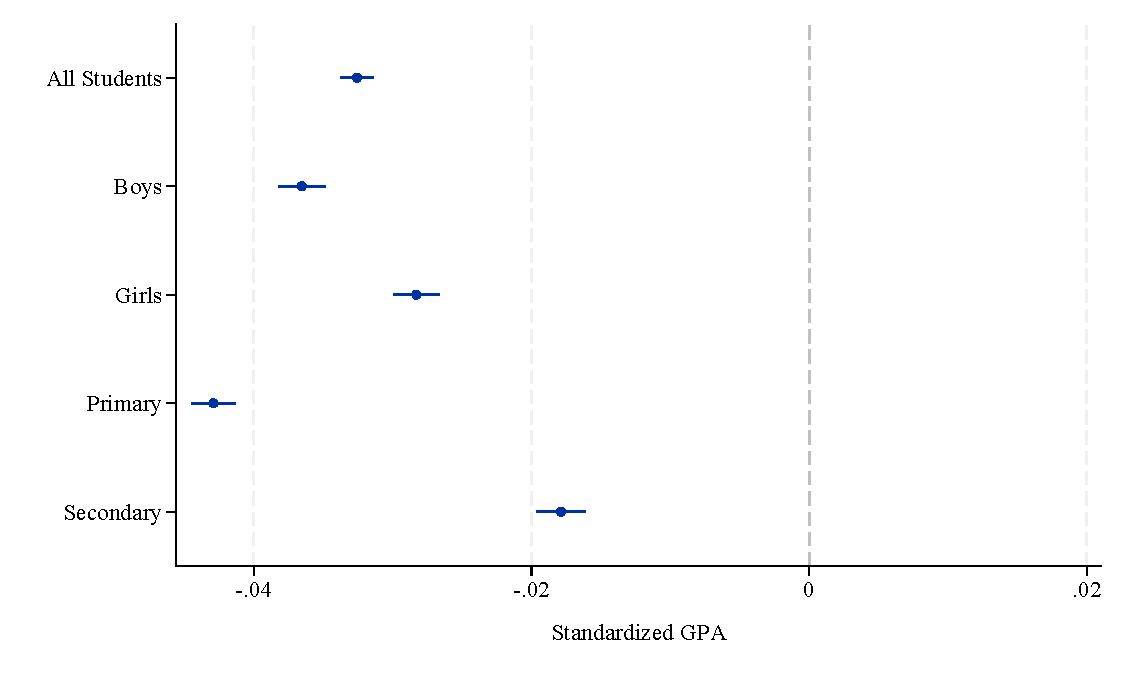
\includegraphics[width=\textwidth]{./FIGURES/TWFE/covid_twfe_B_all_all_gpa_m_adj_4.pdf}
        \caption{Change in gap between children with siblings and only childs}
        \label{fig:fig2b}
    \end{subfigure}
    
    \caption{Learning gap between only childs and siblings}
    \label{fig:fig2}
\end{figure}


\clearpage

%RD-first grade
\makeatletter
\@ifclassloaded{beamer}{%
       \centering
       \resizebox{0.6\textwidth}{!}%
}{%
       \begin{table}[!tbp]\centering\def\sym#1{\ifmmode^{#1}\else\(^{#1}\)\fi}
       \centering
       \caption{Effects of younger sibling delaying school on older sibling standardized exams - 1 - m - a -  - 365}
       \label{tab:rd_summ_1_m_a_365}
       \resizebox{0.95\textwidth}{!}%
}
{
\makeatother
\resizebox{\textwidth}{!}{
\begin{tabular}{lccc}
\toprule
\cmidrule(lr){2-4}
& \multicolumn{3}{c}{Standardized GPA} \\
\cmidrule(lr){2-4}
& Pre-Covid & Covid & Post-Covid  \\
& 2018-2019 & 2020-2021 & 2022-2023  \\
\cmidrule(lr){2-2} \cmidrule(lr){3-3} \cmidrule(lr){4-4}
& (1) & (2) & (3)  \\
\bottomrule
&  &  &   \\
\multirow{2}{*}{\shortstack[l]{Younger sibling born after \\ school-entry cutoff}}&      -0.023***&      -0.001   &      -0.023***\\
                    &     (0.007)   &     (0.007)   &     (0.006)   \\
Local Linear        &         Yes   &         Yes   &         Yes   \\
                    &               &               &               \\
Observations        &     358,861   &     354,044   &     447,536   \\
Counterfactual mean &       0.058   &       0.020   &       0.050   \\
Bandwidth           &         365   &         365   &         365   \\
 

\bottomrule
\end{tabular}
}
\@ifclassloaded{beamer}{%
}{%
       \end{table}
}


\makeatletter
\@ifclassloaded{beamer}{%
       \centering
       \resizebox{0.6\textwidth}{!}%
}{%
       \begin{table}[!tbp]\centering\def\sym#1{\ifmmode^{#1}\else\(^{#1}\)\fi}
       \centering
       \caption{TWFE on 8th grade GPA and standardized exams controlling for baseline 2nd grade standardized exams}
       \label{tab:twfe_ece}
       \resizebox{0.95\textwidth}{!}%
}
{
\makeatother
\begin{tabular}{lcccc}
\toprule
\cmidrule(lr){2-5}
& \multicolumn{4}{c}{TWFE} \\
\cmidrule(lr){2-5}
& 1-3 siblings & 1 sibling & 2 siblings & 3 siblings  \\
\cmidrule(lr){2-2} \cmidrule(lr){3-3} \cmidrule(lr){4-4} \cmidrule(lr){5-5}
& (1) & (2) & (3) & (4) \\
\bottomrule
&  &  & &  \\
&  &  & &  \\
\multicolumn{5}{l}{Panel A: GPA } \\
Mathematics         &      -0.099***&      -0.011   &      -0.036***&      -0.059***\\
                    &     (0.009)   &     (0.009)   &     (0.011)   &     (0.015)   \\
                    &               &               &               &               \\
Observations        &     326,669   &     279,833   &     225,092   &     179,575   \\
 
&  &  & &  \\
Reading             &      -0.099***&      -0.010   &      -0.031***&      -0.034** \\
                    &     (0.009)   &     (0.009)   &     (0.010)   &     (0.015)   \\
                    &               &               &               &               \\
Observations        &     326,669   &     280,846   &     225,840   &     180,218   \\
 
&  &  & &  \\
\multicolumn{5}{l}{Panel B: Standardized Exams } \\
Mathematics         &      -0.034***&      -0.017** &      -0.044***&      -0.071***\\
                    &     (0.006)   &     (0.007)   &     (0.008)   &     (0.011)   \\
                    &               &               &               &               \\
Observations        &     409,527   &     282,640   &     227,403   &     181,370   \\
 
&  &  & &  \\
Reading             &      -0.013** &       0.002   &      -0.022***&      -0.046***\\
                    &     (0.006)   &     (0.006)   &     (0.008)   &     (0.011)   \\
                    &               &               &               &               \\
Observations        &     409,690   &     282,769   &     227,486   &     181,466   \\
 

\bottomrule
\end{tabular}
}
\@ifclassloaded{beamer}{%
}{%
       \end{table}
}

\makeatletter
\@ifclassloaded{beamer}{%
       \centering
       \resizebox{0.6\textwidth}{!}%
}{%
       \begin{table}[!tbp]\centering\def\sym#1{\ifmmode^{#1}\else\(^{#1}\)\fi}
       \centering
       \caption{TWFE on GPA controlling for baseline standardized exams}
       \label{tab:twfe_ece_survey_1}
       \resizebox{0.7\textwidth}{!}%
}
{
\makeatother
\begin{tabular}{lcccc}
\toprule
\cmidrule(lr){2-5}
& \multicolumn{4}{c}{TWFE} \\
\cmidrule(lr){2-5}
& 1-3 siblings & 1 sibling & 2 siblings & 3 siblings  \\
\cmidrule(lr){2-2} \cmidrule(lr){3-3} \cmidrule(lr){4-4} \cmidrule(lr){5-5}
& (1) & (2) & (3) & (4) \\
\bottomrule
&  &  & &  \\
&  &  & &  \\
\multicolumn{5}{l}{Panel A: All studentes } \\
Mathematics         &      -0.041***&      -0.024***&      -0.059***&      -0.082***\\
                    &     (0.003)   &     (0.003)   &     (0.004)   &     (0.005)   \\
 
&  &  & &  \\
Reading             &      -0.037***&      -0.024***&      -0.054***&      -0.066***\\
                    &     (0.003)   &     (0.003)   &     (0.004)   &     (0.005)   \\
                    &               &               &               &               \\
Observations        &   2,211,093   &   1,600,804   &   1,284,541   &   1,025,013   \\
 
&  &  & &  \\
\multicolumn{5}{l}{Panel B: Low SES Households (Q1)} \\
Mathematics         &      -0.028***&      -0.009   &      -0.036***&      -0.061***\\
                    &     (0.005)   &     (0.006)   &     (0.006)   &     (0.008)   \\
 
&  &  & &  \\
Reading             &      -0.022***&      -0.010   &      -0.029***&      -0.044***\\
                    &     (0.005)   &     (0.006)   &     (0.007)   &     (0.008)   \\
                    &               &               &               &               \\
Observations        &     643,621   &     398,084   &     358,488   &     290,244   \\
 
&  &  & &  \\
\multicolumn{5}{l}{Panel C: High SES Households (Q4)} \\
Mathematics         &      -0.035***&      -0.029***&      -0.051***&      -0.072***\\
                    &     (0.006)   &     (0.007)   &     (0.009)   &     (0.019)   \\
 
&  &  & &  \\
Reading             &      -0.039***&      -0.032***&      -0.068***&      -0.010   \\
                    &     (0.006)   &     (0.007)   &     (0.010)   &     (0.019)   \\
                    &               &               &               &               \\
Observations        &     385,616   &     318,633   &     230,174   &     186,296   \\
 
&  &  & &  \\
\multicolumn{5}{l}{Panel D: Households with no PC or Internet} \\
Mathematics         &      -0.037***&      -0.024***&      -0.067***&      -0.089***\\
                    &     (0.005)   &     (0.005)   &     (0.006)   &     (0.010)   \\
 
&  &  & &  \\
Reading             &      -0.036***&      -0.025***&      -0.063***&      -0.083***\\
                    &     (0.005)   &     (0.005)   &     (0.006)   &     (0.010)   \\
                    &               &               &               &               \\
Observations        &     766,875   &     566,628   &     447,252   &     356,075   \\
 
&  &  & &  \\
\multicolumn{5}{l}{Panel E: Households with both PC and Internet} \\
Mathematics         &      -0.043***&      -0.024***&      -0.051***&      -0.080***\\
                    &     (0.005)   &     (0.005)   &     (0.006)   &     (0.008)   \\
 
&  &  & &  \\
Reading             &      -0.035***&      -0.018***&      -0.049***&      -0.054***\\
                    &     (0.005)   &     (0.005)   &     (0.006)   &     (0.008)   \\
                    &               &               &               &               \\
Observations        &     793,797   &     552,557   &     452,886   &     360,214   \\
 

\bottomrule
\end{tabular}
}
\@ifclassloaded{beamer}{%
}{%
       \end{table}
}

\makeatletter
\@ifclassloaded{beamer}{%
       \centering
       \resizebox{0.6\textwidth}{!}%
}{%
       \begin{table}[!tbp]\centering\def\sym#1{\ifmmode^{#1}\else\(^{#1}\)\fi}
       \centering
       \caption{TWFE on GPA controlling for baseline standardized exams}
       \resizebox{0.95\textwidth}{!}%
}
{
\makeatother
\begin{tabular}{lcccc}
\toprule
\cmidrule(lr){2-5}
& \multicolumn{4}{c}{TWFE} \\
\cmidrule(lr){2-5}
& 1-3 siblings & 1 sibling & 2 siblings & 3 siblings  \\
\cmidrule(lr){2-2} \cmidrule(lr){3-3} \cmidrule(lr){4-4} \cmidrule(lr){5-5}
& (1) & (2) & (3) & (4) \\
\bottomrule
&  &  & &  \\
&  &  & &  \\
\multicolumn{5}{l}{Panel A: All studentes } \\
Mathematics         &      -0.041***&      -0.024***&      -0.059***&      -0.082***\\
                    &     (0.003)   &     (0.003)   &     (0.004)   &     (0.005)   \\
                    &               &               &               &               \\
Observations        &   2,225,341   &   1,611,033   &   1,292,849   &   1,031,572   \\
 
&  &  & &  \\
Reading             &      -0.041***&      -0.024***&      -0.059***&      -0.082***\\
                    &     (0.003)   &     (0.003)   &     (0.004)   &     (0.005)   \\
                    &               &               &               &               \\
Observations        &   2,225,341   &   1,611,033   &   1,292,849   &   1,031,572   \\
 
&  &  & &  \\
\multicolumn{5}{l}{Panel B: Parents or students don't expect to graduate from school} \\
Mathematics         &      -0.065***&      -0.047*  &      -0.106***&      -0.104***\\
                    &     (0.020)   &     (0.024)   &     (0.027)   &     (0.037)   \\
                    &               &               &               &               \\
Observations        &      49,164   &      30,696   &      25,807   &      19,899   \\
 
&  &  & &  \\
Reading             &      -0.065***&      -0.047*  &      -0.106***&      -0.104***\\
                    &     (0.020)   &     (0.024)   &     (0.027)   &     (0.037)   \\
                    &               &               &               &               \\
Observations        &      49,164   &      30,696   &      25,807   &      19,899   \\
 
&  &  & &  \\
\multicolumn{5}{l}{Panel C: Parents or students expect to finish 4-year college education} \\
Mathematics         &      -0.045***&      -0.029***&      -0.064***&      -0.091***\\
                    &     (0.003)   &     (0.003)   &     (0.004)   &     (0.006)   \\
                    &               &               &               &               \\
Observations        &   1,759,401   &   1,300,975   &   1,023,717   &     812,634   \\
 
&  &  & &  \\
Reading             &      -0.045***&      -0.029***&      -0.064***&      -0.091***\\
                    &     (0.003)   &     (0.003)   &     (0.004)   &     (0.006)   \\
                    &               &               &               &               \\
Observations        &   1,759,401   &   1,300,975   &   1,023,717   &     812,634   \\
 

\bottomrule
\end{tabular}
}
\@ifclassloaded{beamer}{%
}{%
       \end{table}
}





\makeatletter
\@ifclassloaded{beamer}{%
       \centering
       \resizebox{0.6\textwidth}{!}%
}{%
       \begin{table}[!tbp]\centering\def\sym#1{\ifmmode^{#1}\else\(^{#1}\)\fi}
       \centering
       \caption{Effects of younger sibling delaying school on older sibling standardized exams and parental investment}
       \label{tab:rd_ece_index_365}
       \resizebox{0.95\textwidth}{!}%
}
{
\makeatother
\begin{tabular}{lccccc}
\toprule
& \multicolumn{2}{c}{Pre-Covid}  & \multicolumn{3}{c}{Post-Covid} \\
& \multicolumn{2}{c}{2018-2019}  & \multicolumn{3}{c}{2022-2024}  \\
\cmidrule(lr){2-3} \cmidrule(lr){4-6}
& Mathematics & Reading & Mathematics & Reading & Parental Investment  \\
& (1) & (2) & (3) & (4) & (5) \\
\bottomrule
&  &  &  & &  \\
\multirow{2}{*}{\shortstack[l]{Younger sibling born after \\ school-entry cutoff}}&      -0.025*  &      -0.023*  &      -0.009   &      -0.012   &      -0.035***\\
                    &     (0.014)   &     (0.012)   &     (0.013)   &     (0.010)   &     (0.013)   \\
Local Linear        &         Yes   &         Yes   &         Yes   &         Yes   &         Yes   \\
                    &               &               &               &               &               \\
Observations        &      86,605   &      86,602   &     104,983   &     105,064   &     101,766   \\
Counterfactual mean &      -0.105   &      -0.083   &       0.194   &       0.288   &      -0.004   \\
Bandwidth           &         365   &         365   &         365   &         365   &         365   \\
 

\bottomrule
\end{tabular}
}
\@ifclassloaded{beamer}{%
}{%
       \end{table}
}






